%!TEX root=./report.tex
\section{EVALUATION}

\subsection{Evaluation Metrics}
As a reminder, our task is identifying the correct object model from a large database, given a scan of a model in an uncluttered scene.

We evaluate the correctness of our results with the following metrics:
\begin{itemize}
  \item Percentage of ultimate guesses correct
  \item Confusion matrix for ultimate guess
  \item Precision-recall curve (using registration results)
  \item Average rank of correct model (using voting results)
  \item Area under the cumulative result-within-top-K histogram
\end{itemize}

The results for the Princeton Shape Benchmark can be seen in~\ref{tab:psb_results}
\begin{table}
  \centering
  \begin{tabular}{ | l || c | c | c | c | }
\hline
Metric & PFH & FPFH & SHOT & Spin \\
\hline
 \% Correct & 86.25 & \bf 87.50 & 73.75 & 49.35 \\
AP & 0.85 & \bf 0.86 & 0.64 & 0.31 \\
Avg. Rank & 2.23 & \bf 2.16 & 2.23 & 3.45 \\
AUCR & 0.85 & \bf 0.85 & 0.85 & 0.65 \\
\hline
\end{tabular}
  \caption{Results on the Princeton Shape Benchmark.}
  \label{tab:psb_results}
\end{table}

\begin{figure}[thpb]
\centering
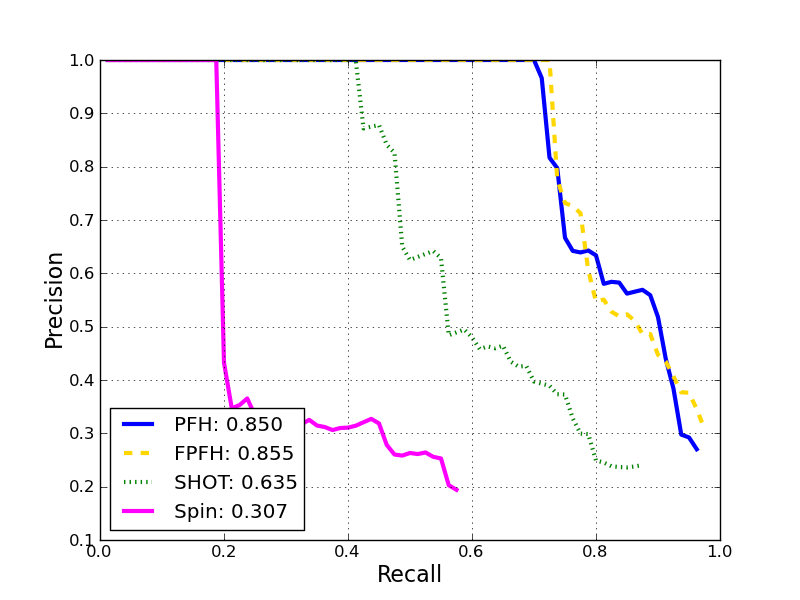
\includegraphics[width=1\linewidth]{../figures/PSB/PFH-FPFH-SHOT-SPIN_IMAGE_pr.png}
\caption{Precision-Recall evaluation of the detectors.}
\label{fig:pr}
\end{figure}


\begin{table*}
\centering
\begin{tabular}{m{0.08\textwidth} m{0.45\textwidth} m{0.45\textwidth}}
  & \begin{center} Confusion Matrix \end{center} & \begin{center} Cumulative Rank Histogram \end{center} \\
  PFH & 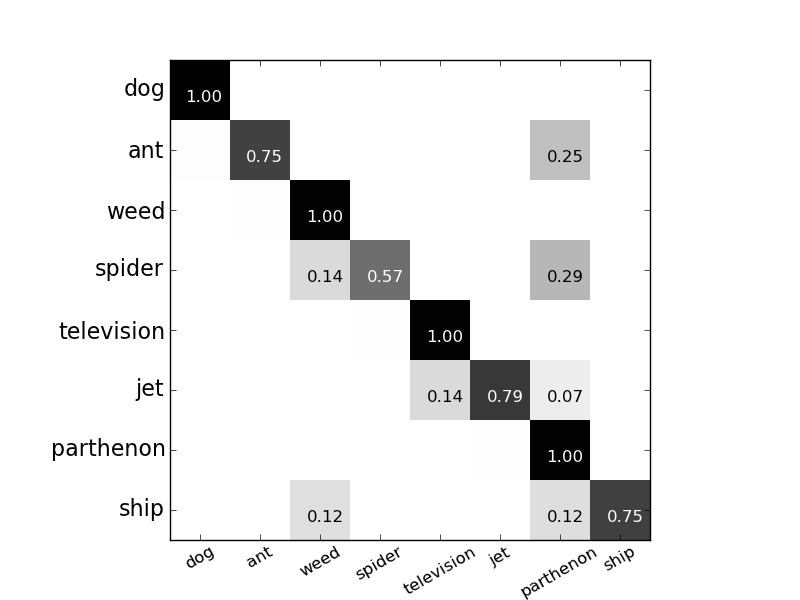
\includegraphics[width=0.45\textwidth,clip=true]{../figures/PSB/PFH_confmat.png} & 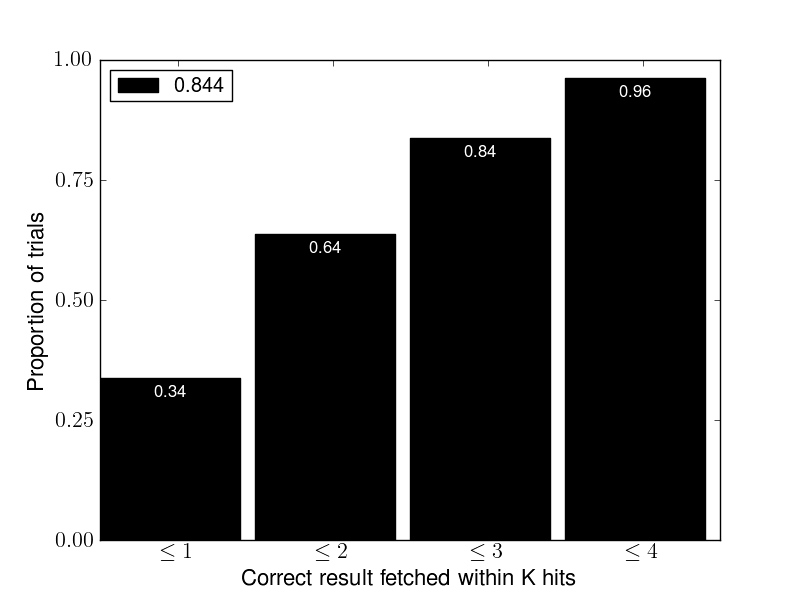
\includegraphics[width=0.45\textwidth,clip=true]{../figures/PSB/PFH_rankhist.png} \\
  FPFH & 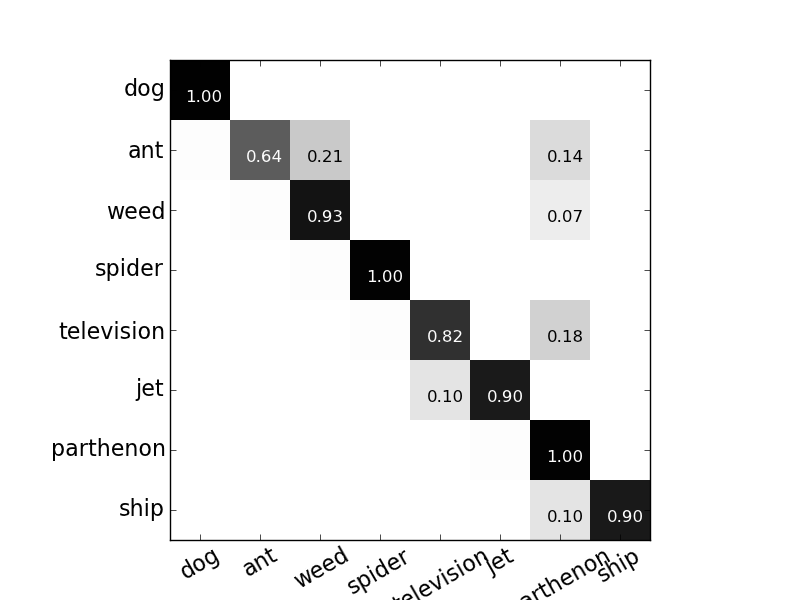
\includegraphics[width=0.45\textwidth,clip=true]{../figures/PSB/FPFH_confmat.png} & 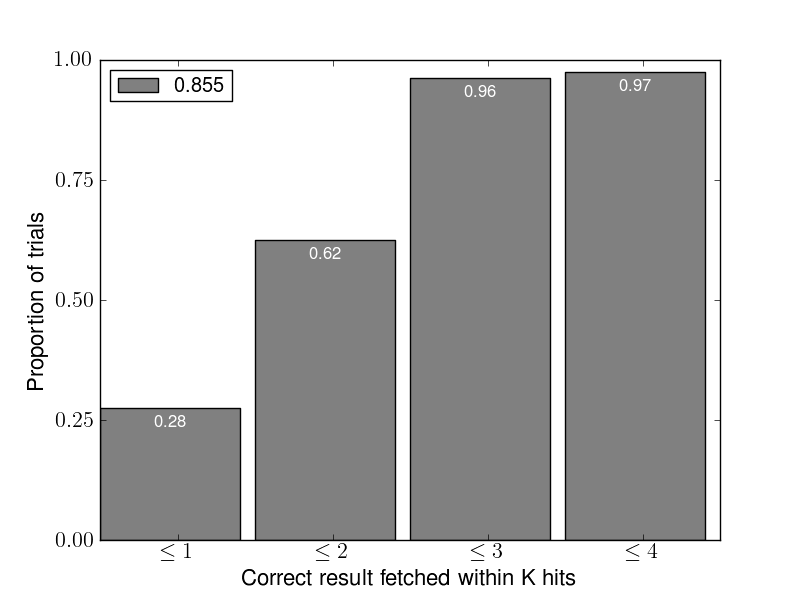
\includegraphics[width=0.45\textwidth,clip=true]{../figures/PSB/FPFH_rankhist.png} \\
  SHOT & 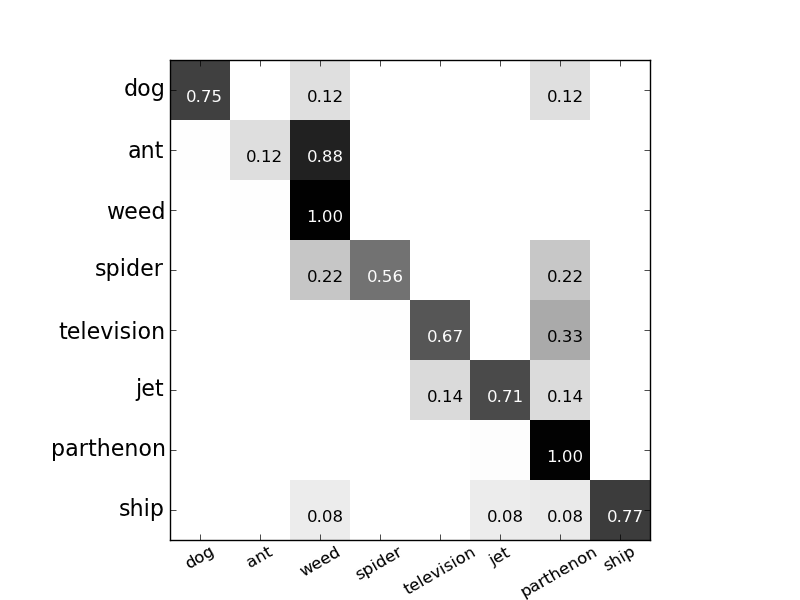
\includegraphics[width=0.45\textwidth,clip=true]{../figures/PSB/SHOT_confmat.png} & 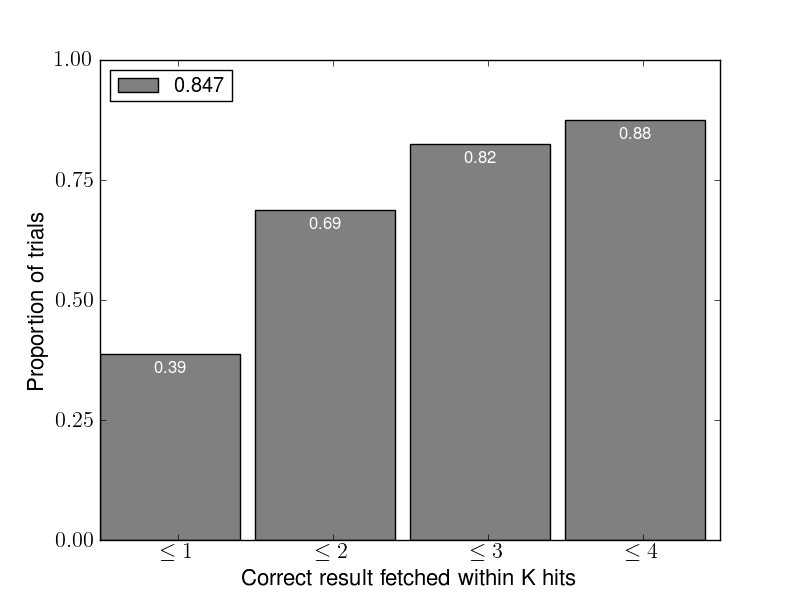
\includegraphics[width=0.45\textwidth,clip=true]{../figures/PSB/SHOT_rankhist.png} \\
  Spin Image & 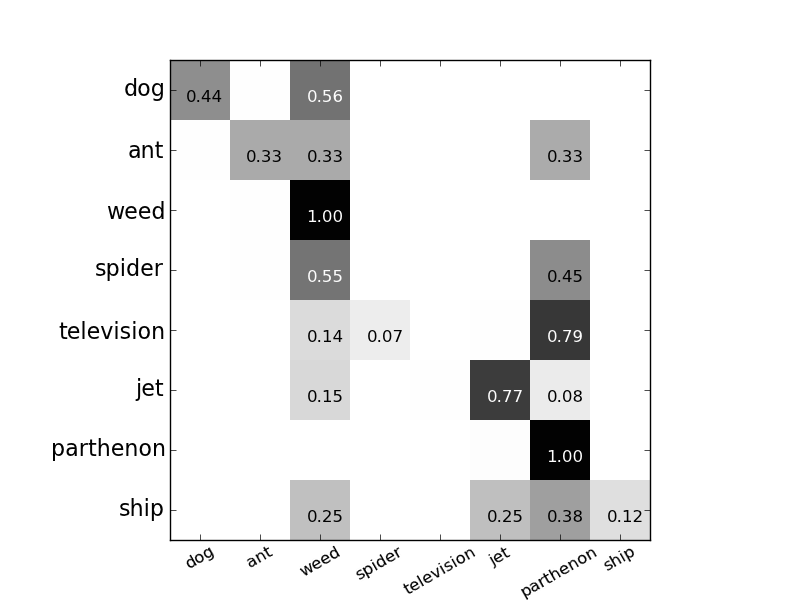
\includegraphics[width=0.45\textwidth,clip=true]{../figures/PSB/SPIN_IMAGE_confmat.png} & 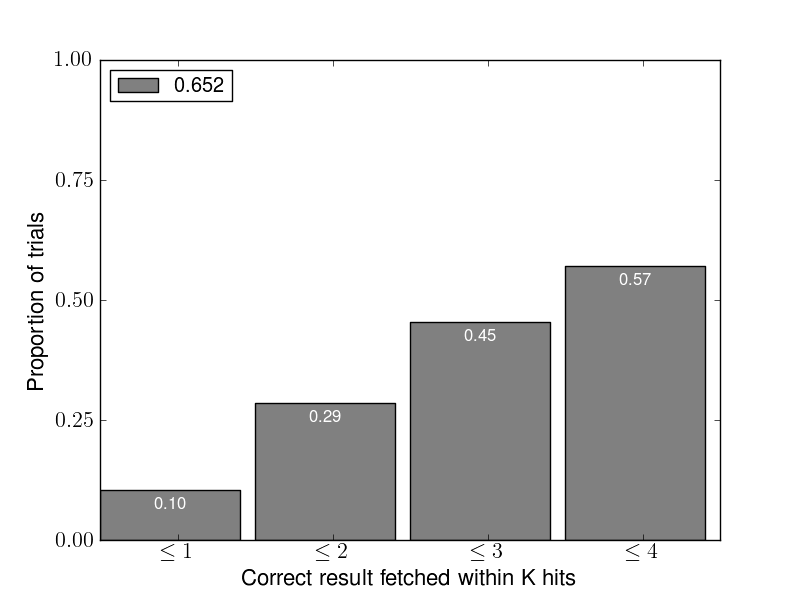
\includegraphics[width=0.45\textwidth,clip=true]{../figures/PSB/SPIN_IMAGE_rankhist.png} \\
\end{tabular}
\caption{A table arranging images}
\label{tab:gt}
\end{table*}

An additional important evaluation is the runtime performance of different methods.
This data allows focused work on fast feature extraction and on algorithms to speed up matching, such as locality-sensitive hashing \cite{Frome2004}.
Hence, we report timing results, split by the different stages of our pipeline, for all experimental conditions.
In all cases, the tests were run on a 2.50 GHz Intel Core2 Quad Q9300 with 4 GB of RAM.

* table per dataset

* features vs. metrics

* plots of the same data that's in the tables?

* confusion matrix figures

* table of timing results
